En la carpeta \texttt{mediciones} se encuentran los archivos de salida correspondientes a cada
experimento. Por cada uno, se adjunta un archivo \texttt{README.txt} con la información conocida
sobre la red en cuestión y otro arhivo \texttt{exceptions.txt} que describe los paquetes sin tipo
capturados. Los nombres de los experimentos denotan el tipo de red, el tipo de conexión y la
duración del experimento en minutos.

\subsubsection{Experimento 1: Red hogareña, cableada, 10 mintos (\texttt{home-eth-10})}

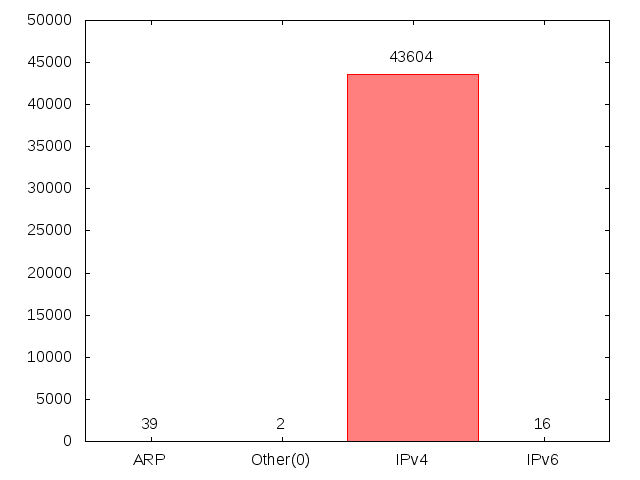
\includegraphics[width=10cm]{../mediciones/home-eth-10/home-eth-10Protocolos.png}

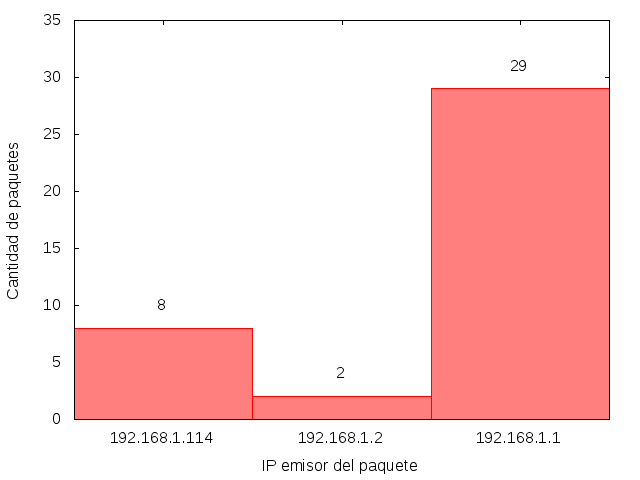
\includegraphics[width=10cm]{../mediciones/home-eth-10/home-eth-10IpsSrcArp.png}

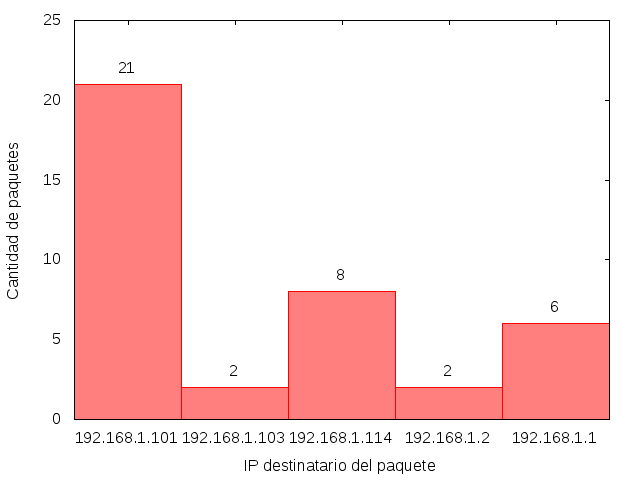
\includegraphics[width=10cm]{../mediciones/home-eth-10/home-eth-10IpsDstArp.png}

\subsubsection{Experimento 2: Red hogareña, inalámbrica, 10 mintos (\texttt{home-wfi-10})}

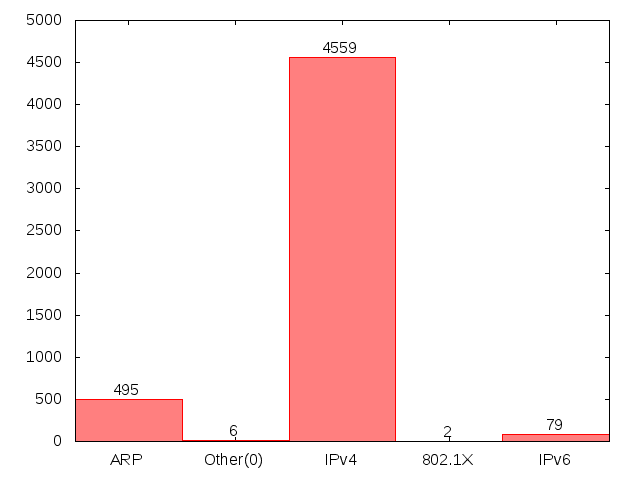
\includegraphics[width=10cm]{../mediciones/home-wfi-10/home-wfi-10Protocolos.png}

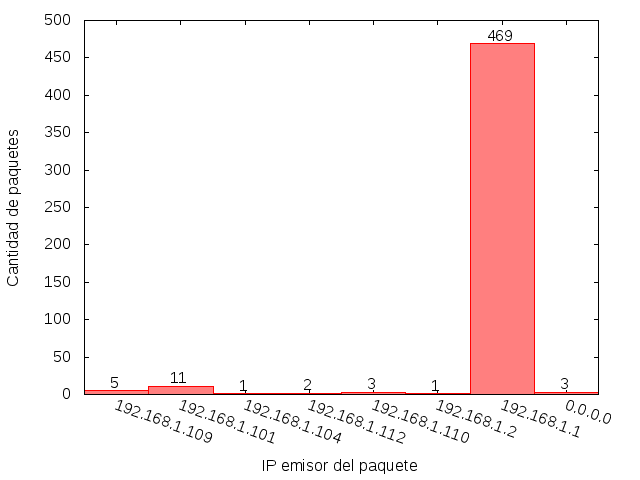
\includegraphics[width=12cm]{../mediciones/home-wfi-10/home-wfi-10IpsSrcArp.png}

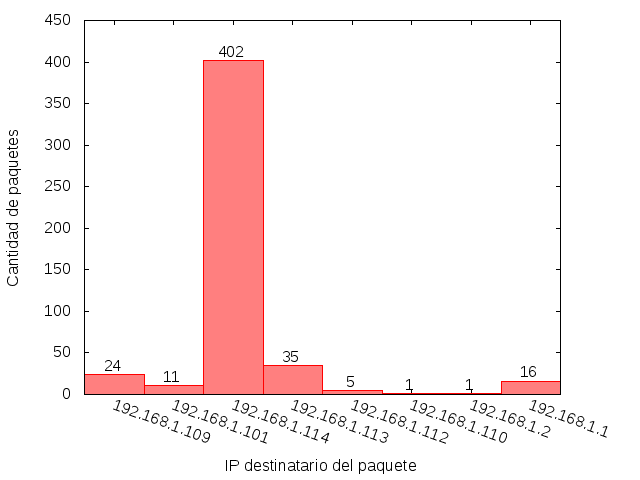
\includegraphics[width=12cm]{../mediciones/home-wfi-10/home-wfi-10IpsDstArp.png}

\subsubsection{Experimento 3: Red pública, inalámbrica, 10 minutos}

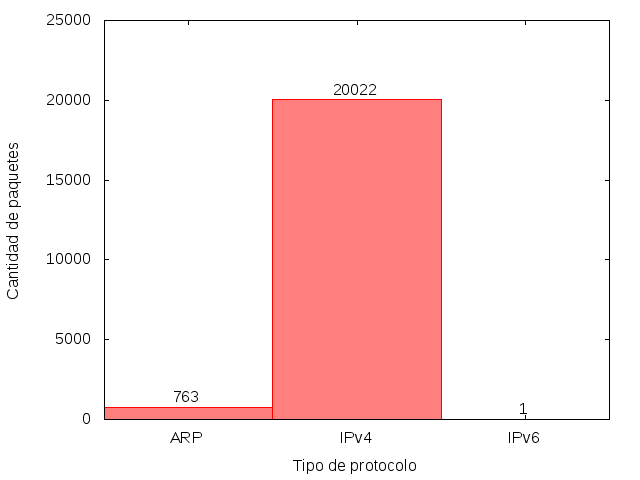
\includegraphics[width=10cm]{../mediciones/altop-wifi-10/altop10Protocolos.png}

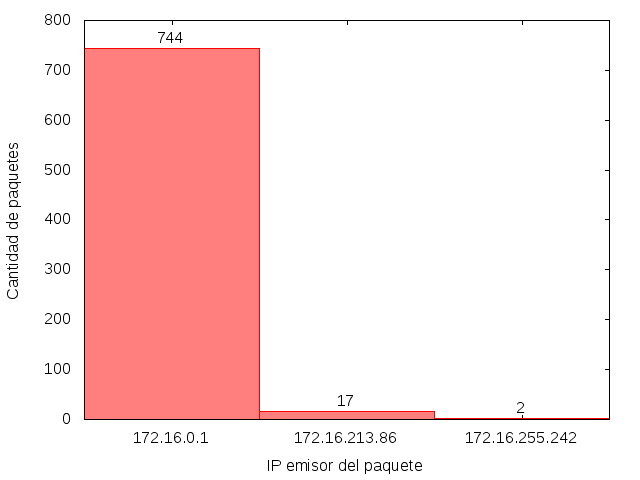
\includegraphics[width=10cm]{../mediciones/altop-wifi-10/altop10IpsSrcArp.png}

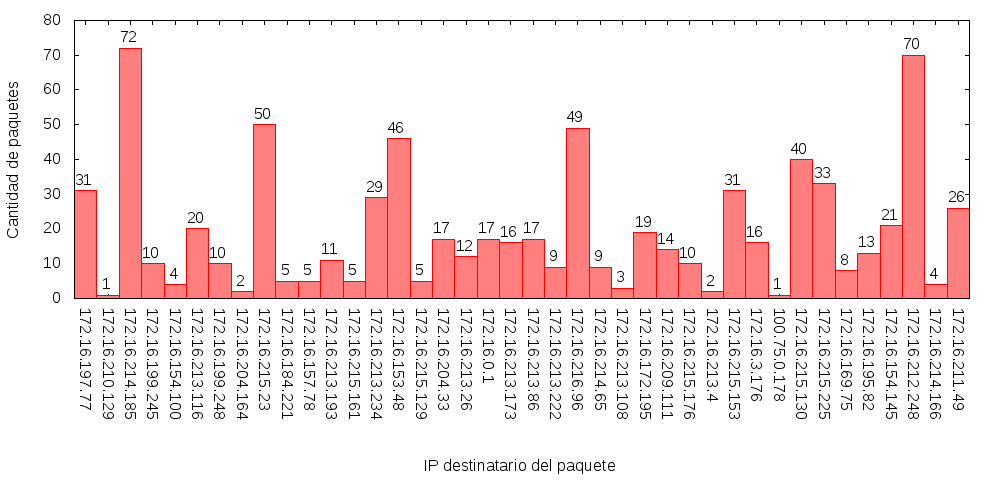
\includegraphics[width=16cm]{../mediciones/altop-wifi-10/altop10IpsDstArp.png}

\subsubsection{Experimento 4: Red pública, inalámbrica, 60 minutos}

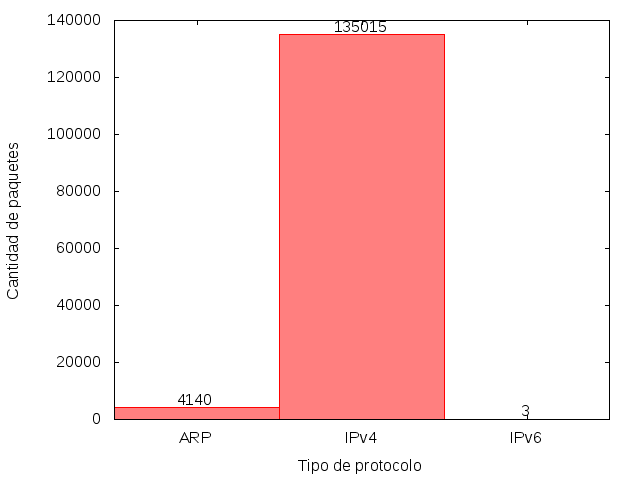
\includegraphics[width=10cm]{../mediciones/altop-wifi-60/altop60Protocolos.png}

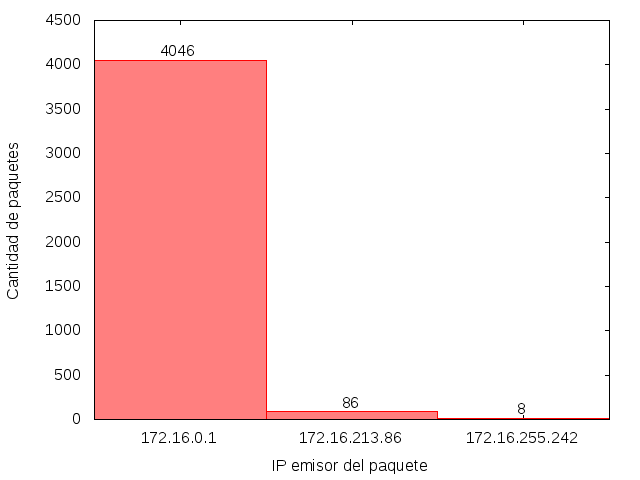
\includegraphics[width=10cm]{../mediciones/altop-wifi-60/altop60IpsSrcArp.png}

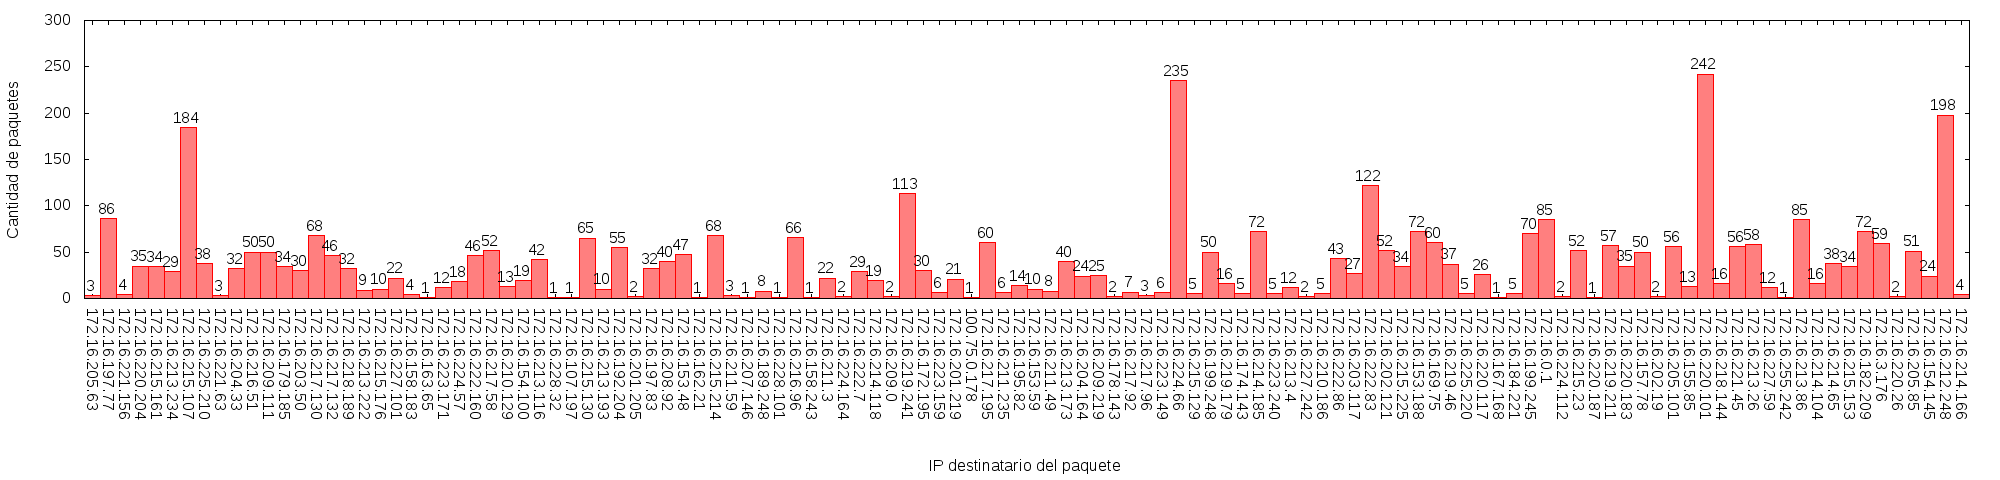
\includegraphics[width=14cm,trim={0 0 35.95cm 0},clip]{../mediciones/altop-wifi-60/altop60IpsDstArp.png}

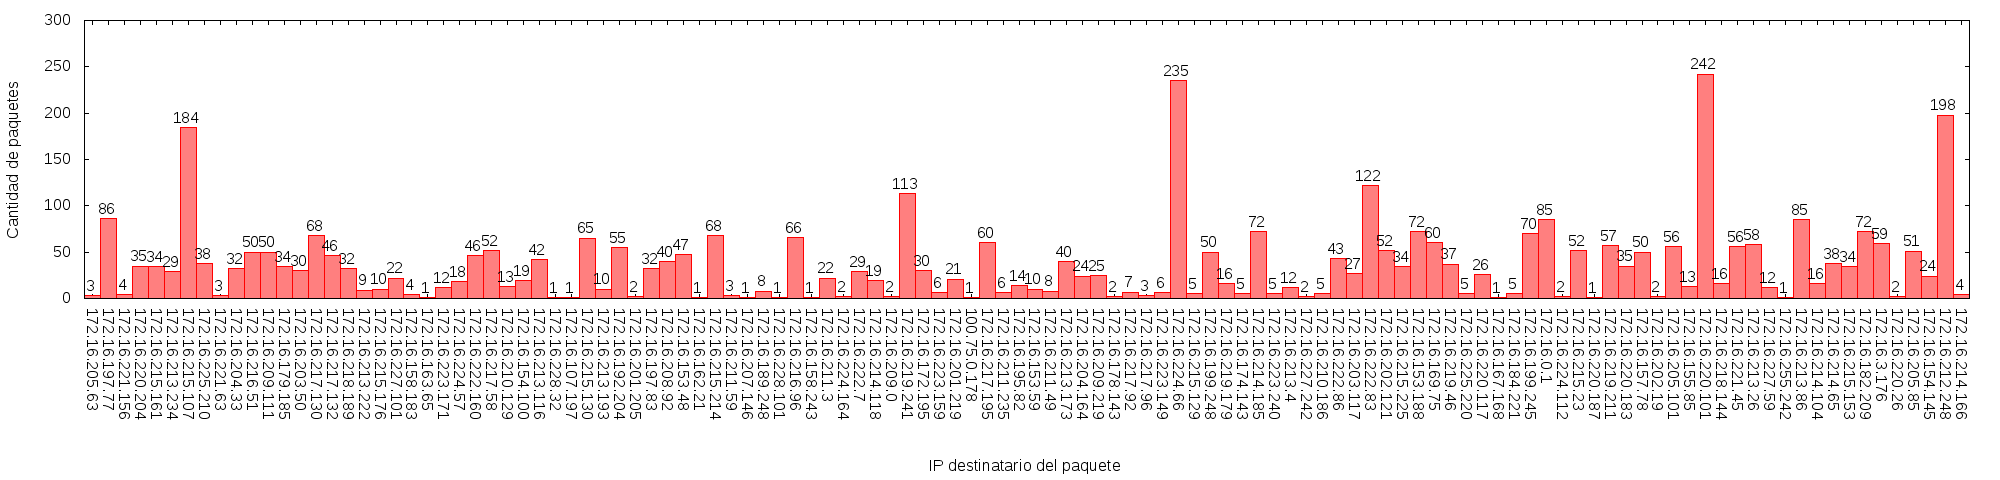
\includegraphics[width=14cm,trim={17cm 0 20.7cm 0},clip]{../mediciones/altop-wifi-60/altop60IpsDstArp.png}

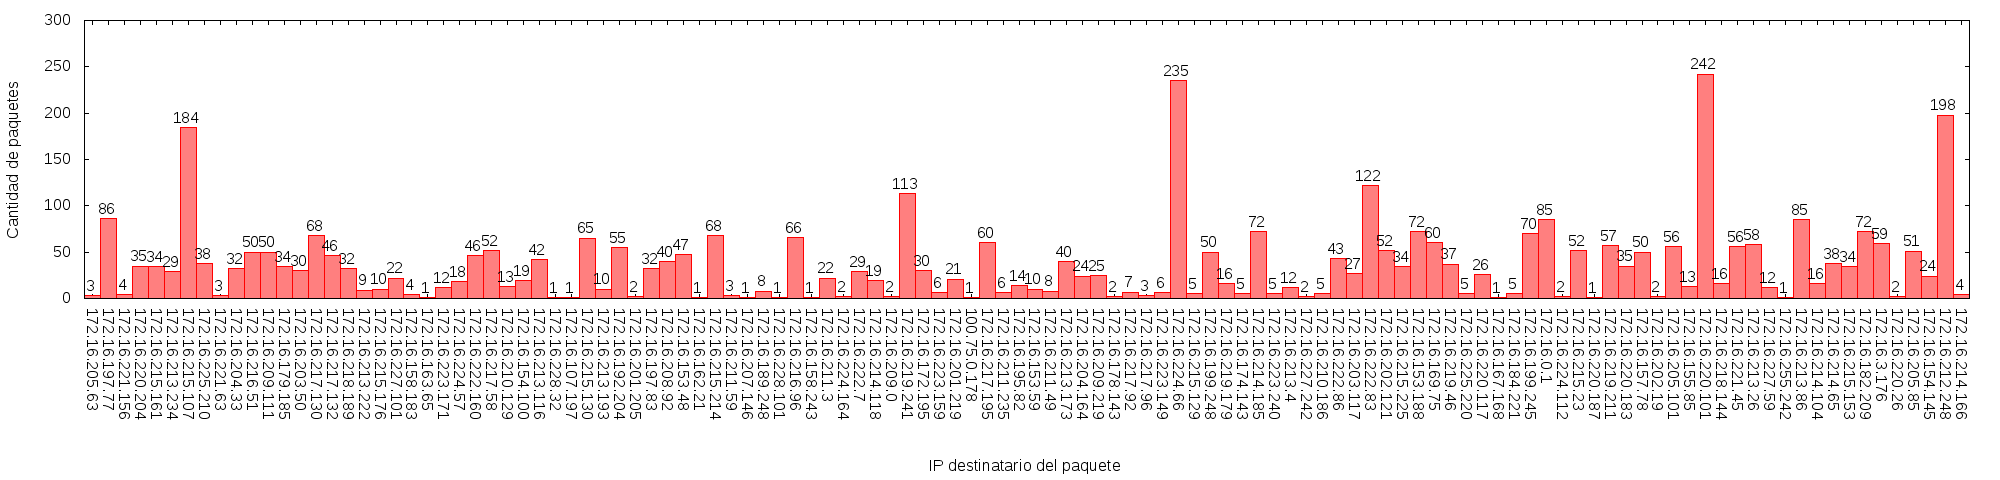
\includegraphics[width=16cm,trim={32.26cm 0 0 0},clip]{../mediciones/altop-wifi-60/altop60IpsDstArp.png}
